\section{Модуль отображения логического времени на физическое}
\indent Так как расчет выполнения операции (как и всей карты технологического процесса) подсистемой имитационного моделирования производится в логическом времени, то есть во времени отсчитываемом от нуля, существует необходимость в отображении (соответствие между элементами двух множеств) логического времени на физическое.
Одной из главных сложностей, возникающих при этом, является неоднородность рабочего времени, которая проявляется в рабочем графике (чередование интервалов рабочего и нерабочего времени), наличии выходных и перенесенных дней.
Другой сложностью является наличие в системе ``обратного расчета'', при котором планирование ведется от даты ``дедлайна'' (дата или время, к которому должна быть выполнена задача), что накладывает свои ограничения на реализацию данной компоненты, такие как:
\begin{itemize}
	\item проблемы с определением рабочих интервалов, которые относятся к текущему дню;
	\item во время обратного расчета происходит движение в другую сторону по оси физического времени;
	\item смещение интервалов рабочего времени относительно рабочего дня.
\end{itemize}
\begin{figure}[h!]
	\centering
	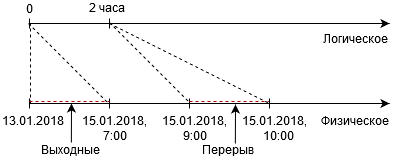
\includegraphics[width=0.8\linewidth]{pics/scheduleAxes.png}
	\caption{Пример отображения оси логического на ось физического времени}
	\label{fig:axes}
\end{figure}

\indent Для отображения логического времени на физическое был предложен итеративный процесс, который осуществляет ``переход'' к необходимому времени путем последовательного перебора дат.\\
\indent Как было сказано ранее, из-за того, что рабочее время не является непрерывным, мы не имеем возможности просуммировать начальную дату и значение поданного логического времени.
Это ведет к тому, что необходимо синхронизировать логическое и физическое время -- это достигается путем последовательного периодического отображения конкретного логического времени на физическое (см. рисунок \ref{fig:axes}).
Это подразумевает под собой наличие двух массивов чисел или ``осей'':

\begin{itemize}
	\item оси логического времени, которая начинается с нуля и единица которой соответствует одной секунде (необходимости в более точном отображении нет);
	\item оси физического времени, на которой может быть отложено любая дата физического времени, отсчет которой начинается 1 января 1970 года 00:00:00 (эпоха Unix).
\end{itemize}

\indent Особенностью оси физического времени является наличие на ней ``выколотых'' точек -- промежутков времени в которые работа не ведется и операции не выполняются.

\indent Входными данными для модуля являются:

\begin{itemize}
	\item дата, с которой необходимо начинать отсчет;
	\item логическое время, которого необходимо достигнуть;
	\item конфигурация, состоящая из данных о рабочем графике, о датах выходных и перенесенных дней.
\end{itemize}

\indent Дата является точкой на физической оси, куда будет отображаться нуль логической. Она представляет собой количество секунд, прошедшее с начала эпохи Unix.

\indent Логическое время~--~количество секунд, которое должно быть отложено на логической оси. В силу непрерывности физической оси, каждой логической точке сопоставляется отрезок на физической оси, сопоставляется пара чисел -- границ данного отрезка.

\begin{lstlisting}[caption={Структуры конфигурации},label={lst:configStruct},language=Golang]
	// WorkInterval : one work interval.
	type WorkInterval struct {
		ShiftID int
		Starts  int64
		Ends    int64
	}
	
	// DayTemplateName : name for day template.
	type DayTemplateName string

	// ScheduleForDay : work intervals for days.
	type ScheduleForDay map[DayTemplateName][]WorkInterval

	// ScheduleTemplate : schedule template for week.
	type ScheduleTemplate [7]DayTemplateName

	// ExceptionDates : exception dates for year.
	type ExceptionDates map[int64]DayTemplateName

	// ConverterConfig : information for mapping logical time to physical.
	type ConverterConfig struct {
		// Weekly schedule template.
		ScheduleTemplate ScheduleTemplate
		// Exception dates for year.
		ExceptionDates ExceptionDates
		// Work intervals for every day.
		ScheduleForDay ScheduleForDay
	}
\end{lstlisting}

\indent Конфигурация модуля~--~данные используемые для определения модулем какие промежутки являются выколотыми точками на оси физического времени.
Состоит из данных о рабочем графике занятого персонала (интервалы рабочего времени), шаблонном расписании на неделю (например, суббота, воскресенье -- выходные, пятница -- ``короткий'' день, остальные -- стандартные рабочие дни), набора информации о датах, которые являются днями-исключениями и соответствующей информацией о графике работы в данные дни.

\begin{figure}[h!]
	\centering
	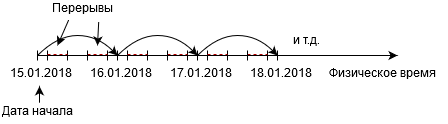
\includegraphics[width=0.7\linewidth]{pics/scheduleStraightCalc.png}
	\caption{Схема прямого расчета}
	\label{fig:straightCalc}
\end{figure}
\begin{figure}[h!]
	\centering
	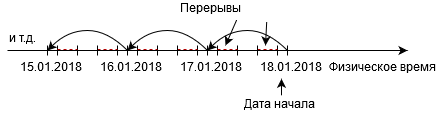
\includegraphics[width=0.7\linewidth]{pics/scheduleReverceCalc.png}
	\caption{Схема обратного расчета}
	\label{fig:reverceCalc}
\end{figure}

\begin{figure}[h!]
	\centering
	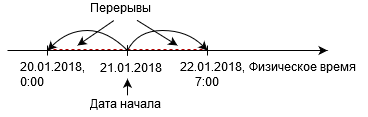
\includegraphics[width=0.7\linewidth]{pics/scheduleCheckCalc.png}
	\caption{Схема проверки времени}
	\label{fig:checkCalc}
\end{figure}

\indent После запуска модуль получает параметры и совершает проверку последних на корректность и непротиворечивость (например, если два дня имеют пересечения временных промежутков, то они противоречивы, ведь ресурс не может работать одновременно в двух сменах) как в рамках смен одного, так соседних дней.
Далее производится определение режима работы: прямой, обратный расчет или проверка времени:

\begin{itemize}
	\item прямой расчет -- задается дата начала отсчета, логическое время и расчет ведется до нахождения даты окончания работ (см рисунок \ref{fig:straightCalc});
	\item обратный расчет -- задается дата дедлайна, логическое время и расчет ведется до нахождения времени начала работ (см рисунок \ref{fig:reverceCalc});
	\item проверка времени -- задается дата и логическое время равное нулю, что запускает оба предыдущих расчета пока не будет найдено первое ненулевое время в обоих направлениях от даты начала расчета (см рисунок \ref{fig:checkCalc}).
\end{itemize}

\begin{figure}[h!]
	\centering
	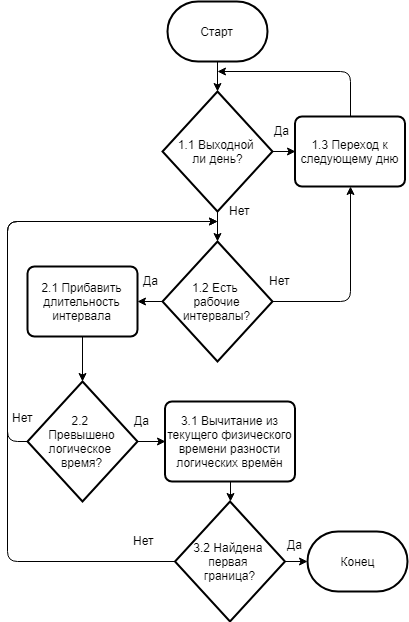
\includegraphics[width=0.7\linewidth]{pics/scheduleSchema.png}
	\caption{Блок-схема модуля}
	\label{fig:schema}
\end{figure}

\indent После выбора режима работы счетчик текущего логического времени обнуляется и счетчик текущего физического времени до стартовой даты. Затем итеративно, пока текущее логическое время не превысит необходимое производится поиск следующей даты.
Алгоритмически поиск даты работает следующим образом (рисунок \ref{fig:schema}):

\begin{enumerate}
	\item[\mylabel{itm:point1}{1})] определяются интервалы рабочих смен относящихся к текущему дню (рисунок \ref{fig:schema}, п. 1.1): при отсутствии таковых (рисунок \ref{fig:schema}, п. 1.2), к текущей дате прибавляется один день и затем возврат к п.\ref{itm:point1} (рисунок \ref{fig:schema}, п. 1.3).
	\item[2)] отсортированные в порядке возрастания интервалы последовательно перебираются и их длительности прибавляются к текущему логическому и физическому времёнам (рисунок \ref{fig:schema}, п. 2.1):
	      \begin{enumerate}
		      \item[а)] при превышении текущим логическим временем необходимого, переход к п.\ref{itm:point3} (рисунок \ref{fig:schema}, п. 2.2);
		      \item[б)] если все интервалы были просуммированы, но необходимое логическое время не превышено -- переход к п.\ref{itm:point1} (рисунок \ref{fig:schema}, п. 2.2);
	      \end{enumerate}
	\item[\mylabel{itm:point3}{3})] разность текущего и необходимого логического времён вычитается из физического времени (рисунок \ref{fig:schema}, п. 3.1), при этом сохраняя данное значение как левую (правую при обратном расчете) границу, после чего продолжается расчет для выявления правой (левой) границы промежутка (рисунок \ref{fig:schema}, п. 3.2).
\end{enumerate}

\indent Определение интервалов рабочего времени происходит взятием даты из текущего физического времени -- затем начинается определение принадлежности данной даты к перенесенным датам после чего есть два варианта:

\begin{itemize}
	\item дата является перенесенным днем и модуль получает информацию о расписании которое нужно применить;
	\item дата не является перенесенным днем и получение информации происходит исходя из того, каким днем недели является данная дата.
\end{itemize}

\begin{figure}[h!]
	\centering
	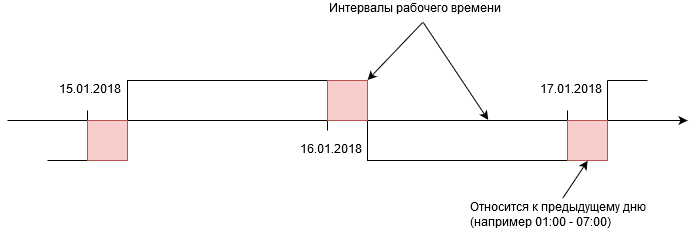
\includegraphics[width=\linewidth]{pics/scheduleIntervals.png}
	\caption{Смещение интервалов рабочего времени относительно рабочего дня}
	\label{fig:intervals}
\end{figure}

\begin{figure}[h!]
	\centering
	
\includegraphics[width=0.6\linewidth]{pics/scheduleTime.png}
	\caption{Граница двух дней}
	\label{fig:time}
\end{figure}

\indent На предприятиях нередко случается так, что рабочие интервалы, принадлежащие к рабочему дню и сам рабочий день смещены относительно друг друга (см. рисунок \ref{fig:intervals}).
При этом возникают трудности с определением интервалов рабочего времени в связи с тем, что для определения используется количество секунд с начала эпохи Unix и до нуля часов нуля минут и нуля секунд нужной даты.
По количеству секунд, используя инструментарий языка, определяется каким днем недели является нужная дата и, соответственно, по дню недели задается шаблон рабочего дня.
Эти трудности практически не влияют на прямой расчет, но с обратным все немного сложнее.
Так как в одном дне 86400 секунд и, если рассматривать границу двух дней (см. рисунок \ref{fig:time}), то 86400 секунда предыдущего дня будет равна нулевой секунде нового дня.
Можно сказать, что 86400 -- левый предел, а 0 -- правый предел в данной точке (особенно, если изображать в виде окружности).
Но, в связи с тем, что данная недетерминированность присутствует лишь при рассмотрении ситуации человеком, а система может распознавать диапазон от 0 до 86399 секунд.
Тогда, в качестве решения данной проблемы, для определения интервалов рабочего графика (при обратном расчете) используется величина в 86399 секунд, как последняя секунда текущего дня, при условии, что данное допущение не влияет на расчет.

% \begin{figure}[h!]
% 	\centering
% 	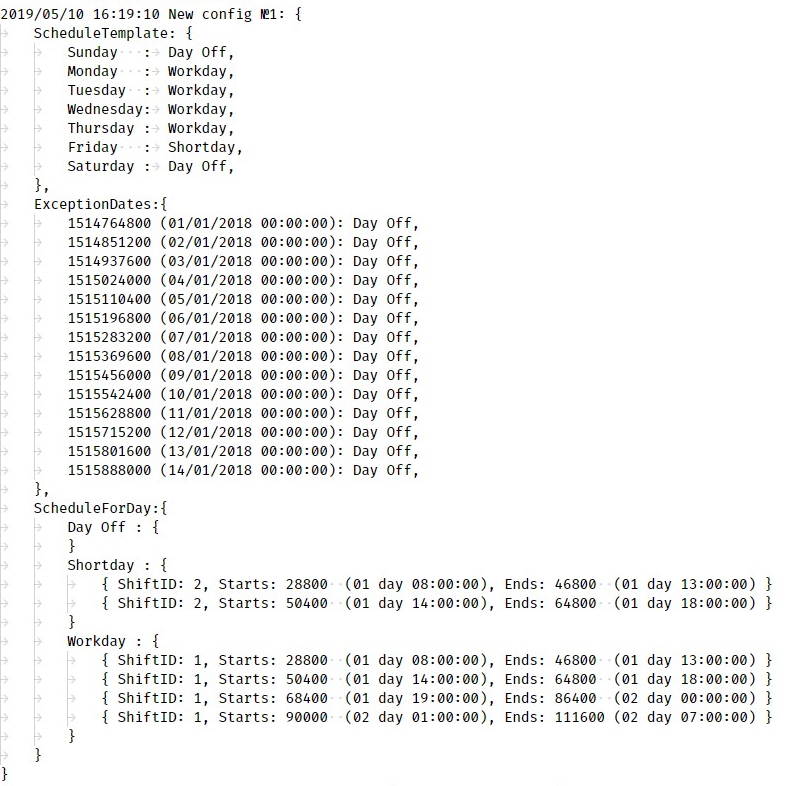
\includegraphics[scale=0.6]{pics/scheduleConfigExample.png}
% 	\caption{Пример конфигурации модуля}
% 	\label{fig:config}
% \end{figure}

\begin{lstlisting}[caption={Пример прямого расчета модулем},label={lst:config}]
	2019/05/31 16:01:23 New config 1: {
		ScheduleTemplate: {
			Sunday   :	Day Off,
			Monday   :	Workday,
			Tuesday  :	Workday,
			Wednesday:	Workday,
			Thursday :	Workday,
			Friday   :	Shortday,
			Saturday :	Day Off,
		},
		ExceptionDates:{
			1514764800 (01/01/2018 00:00:00): Day Off,
			1514851200 (02/01/2018 00:00:00): Day Off,
			1514937600 (03/01/2018 00:00:00): Day Off,
			1515024000 (04/01/2018 00:00:00): Day Off,
			1515110400 (05/01/2018 00:00:00): Day Off,
			1515196800 (06/01/2018 00:00:00): Day Off,
			1515283200 (07/01/2018 00:00:00): Day Off,
			1515369600 (08/01/2018 00:00:00): Day Off,
			1515456000 (09/01/2018 00:00:00): Day Off,
			1515542400 (10/01/2018 00:00:00): Day Off,
			1515628800 (11/01/2018 00:00:00): Day Off,
			1515715200 (12/01/2018 00:00:00): Day Off,
			1515801600 (13/01/2018 00:00:00): Day Off,
			1515888000 (14/01/2018 00:00:00): Day Off,
		},
		ScheduleForDay:{
			Day Off : {
			}
			Shortday : {
				{ ShiftID: 2, Starts: 28800  (01 day 08:00:00), Ends: 46800  (01 day 13:00:00) }
				{ ShiftID: 2, Starts: 50400  (01 day 14:00:00), Ends: 64800  (01 day 18:00:00) }
			}
			Workday : {
				{ ShiftID: 1, Starts: 28800  (01 day 08:00:00), Ends: 46800  (01 day 13:00:00) }
				{ ShiftID: 1, Starts: 50400  (01 day 14:00:00), Ends: 64800  (01 day 18:00:00) }
				{ ShiftID: 1, Starts: 68400  (01 day 19:00:00), Ends: 86400  (02 day 00:00:00) }
				{ ShiftID: 1, Starts: 90000  (02 day 01:00:00), Ends: 111600 (02 day 07:00:00) }
			}
		}
	}
\end{lstlisting}

\indent Возвращаясь к пункту \ref{itm:point3} алгоритма при нахождении нужного времени работа модуля не прекращается, а ведется до момента нахождения второй границы промежутка, на который отображается необходимое логической время.

\indent Как было сказано ранее -- физическое время непрерывно, а следовательно когда производится отображение на него логического времени, в результате получается промежуток (см. рисунок \ref{fig:axes}), который и характеризуют две границы.
Эта пара чисел, характеризующая начало и конец отрезка, которые отображаются на логическую ось в точке, где значение равно входному логическому времени и являются выходными данными данного модуля.

% \begin{figure}[ht!]
% 	\centering
% 	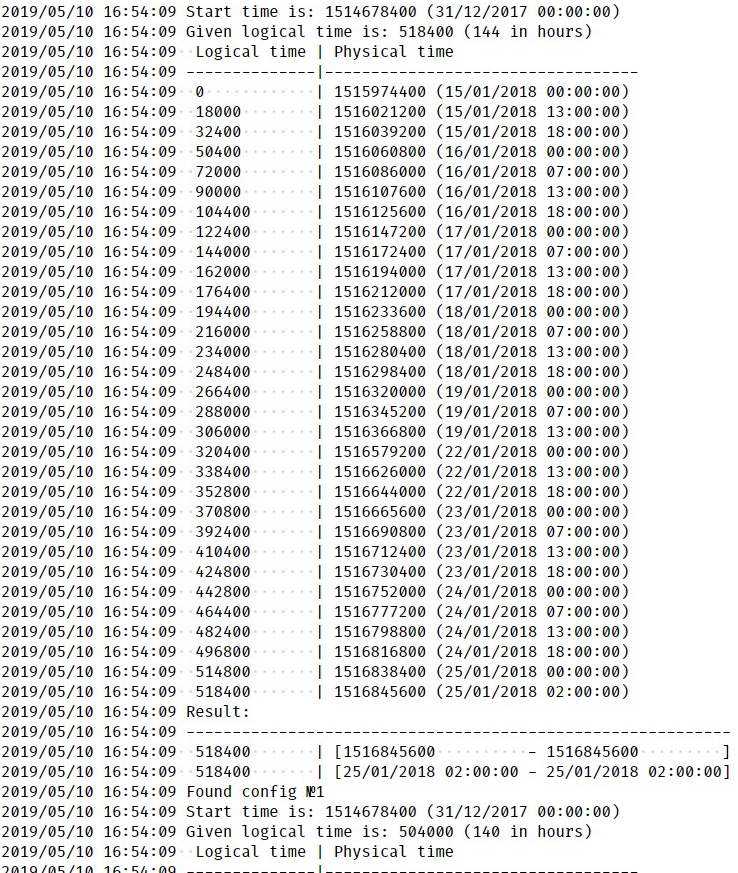
\includegraphics[scale=0.6]{pics/scheduleEvalExample.png}
% 	\caption{Пример прямого расчета модулем}
% 	\label{fig:eval1}
% \end{figure}
\begin{lstlisting}[caption={Пример прямого расчета модулем},label={lst:eval1}]
	2019/05/31 15:10:50 Start time is: 1514678400 (31/12/2017 00:00:00)
	2019/05/31 15:10:50 Given logical time is: 518400 (144 in hours)
	2019/05/31 15:10:50  Logical time | Physical time
	2019/05/31 15:10:50 --------------|----------------------------------
	2019/05/31 15:10:50  0            | 1515974400 (15/01/2018 00:00:00)
	2019/05/31 15:10:50  18000        | 1516021200 (15/01/2018 13:00:00)
	2019/05/31 15:10:50  32400        | 1516039200 (15/01/2018 18:00:00)
	2019/05/31 15:10:50  50400        | 1516060800 (16/01/2018 00:00:00)
	2019/05/31 15:10:50  72000        | 1516086000 (16/01/2018 07:00:00)
	2019/05/31 15:10:50  90000        | 1516107600 (16/01/2018 13:00:00)
	2019/05/31 15:10:50  104400       | 1516125600 (16/01/2018 18:00:00)
	2019/05/31 15:10:50  122400       | 1516147200 (17/01/2018 00:00:00)
	2019/05/31 15:10:50  144000       | 1516172400 (17/01/2018 07:00:00)
	2019/05/31 15:10:50  162000       | 1516194000 (17/01/2018 13:00:00)
	2019/05/31 15:10:50  176400       | 1516212000 (17/01/2018 18:00:00)
	2019/05/31 15:10:50  194400       | 1516233600 (18/01/2018 00:00:00)
	2019/05/31 15:10:50  216000       | 1516258800 (18/01/2018 07:00:00)
	2019/05/31 15:10:50  234000       | 1516280400 (18/01/2018 13:00:00)
	2019/05/31 15:10:50  248400       | 1516298400 (18/01/2018 18:00:00)
	2019/05/31 15:10:50  266400       | 1516320000 (19/01/2018 00:00:00)
	2019/05/31 15:10:50  288000       | 1516345200 (19/01/2018 07:00:00)
	2019/05/31 15:10:50  306000       | 1516366800 (19/01/2018 13:00:00)
	2019/05/31 15:10:50  320400       | 1516579200 (22/01/2018 00:00:00)
	2019/05/31 15:10:50  338400       | 1516626000 (22/01/2018 13:00:00)
	2019/05/31 15:10:50  352800       | 1516644000 (22/01/2018 18:00:00)
	2019/05/31 15:10:50  370800       | 1516665600 (23/01/2018 00:00:00)
	2019/05/31 15:10:50  392400       | 1516690800 (23/01/2018 07:00:00)
	2019/05/31 15:10:50  410400       | 1516712400 (23/01/2018 13:00:00)
	2019/05/31 15:10:50  424800       | 1516730400 (23/01/2018 18:00:00)
	2019/05/31 15:10:50  442800       | 1516752000 (24/01/2018 00:00:00)
	2019/05/31 15:10:50  464400       | 1516777200 (24/01/2018 07:00:00)
	2019/05/31 15:10:50  482400       | 1516798800 (24/01/2018 13:00:00)
	2019/05/31 15:10:50  496800       | 1516816800 (24/01/2018 18:00:00)
	2019/05/31 15:10:50  514800       | 1516838400 (25/01/2018 00:00:00)
	2019/05/31 15:10:50  518400       | 1516845600 (25/01/2018 02:00:00)
	2019/05/31 15:10:50 Result:
	2019/05/31 15:10:50 -----------------------------------------------------------
	2019/05/31 15:10:50  518400  | [1516845600          - 1516845600         ]
	2019/05/31 15:10:50  518400  | [25/01/2018 02:00:00 - 25/01/2018 02:00:00]
	--- PASS: TestOffsetToTimeLine (0.08s)
	PASS
	ok  	nitta.io/yamp/schedule	0.860s
	Success: Tests passed.
\end{lstlisting}

\indent В результате работы над модулем было проведено тестирование, результаты одного из которых можно увидеть на листингах \ref{lst:config} и \ref{lst:eval1}.
На листинге \ref{lst:config} приведена конфигурация модуля, которая показывает, как производится совмещение логического и физического дня, обработка перенесенных дней.
На листинге \ref{lst:eval1}, перед расчетом нового отображения, можно отметить, что при использовании той же конфигурации не производится ее повторный вывод в журнал, что позволяет сократить его длину, а следовательно улучшить читаемость.
Листинг \ref{lst:eval1} показывает итеративный процесс как результат прибавления каждого нового интервала к текущему времени.

% \begin{figure}[ht!]
% 	\centering
% 	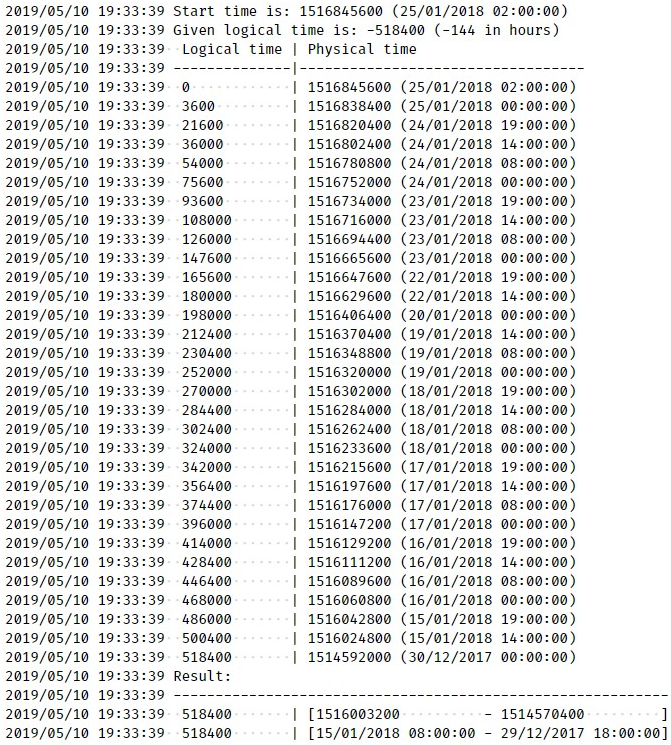
\includegraphics[scale=0.6]{pics/scheduleRevertEvalExample.png}
% 	\caption{Пример обратного расчета модулем}
% 	\label{fig:revEval}
% \end{figure}
\begin{lstlisting}[caption={Пример обратного расчета модулем},label={lst:revEval}]
	2019/05/31 15:09:35 Start time is: 1516845600 (25/01/2018 02:00:00)
	2019/05/31 15:09:35 Given logical time is: -518400 (-144 in hours)
	2019/05/31 15:09:35  Logical time | Physical time
	2019/05/31 15:09:35 --------------|----------------------------------
	2019/05/31 15:09:35  0            | 1516845600 (25/01/2018 02:00:00)
	2019/05/31 15:09:35  3600         | 1516838400 (25/01/2018 00:00:00)
	2019/05/31 15:09:35  21600        | 1516820400 (24/01/2018 19:00:00)
	2019/05/31 15:09:35  36000        | 1516802400 (24/01/2018 14:00:00)
	2019/05/31 15:09:35  54000        | 1516780800 (24/01/2018 08:00:00)
	2019/05/31 15:09:35  75600        | 1516752000 (24/01/2018 00:00:00)
	2019/05/31 15:09:35  93600        | 1516734000 (23/01/2018 19:00:00)
	2019/05/31 15:09:35  108000       | 1516716000 (23/01/2018 14:00:00)
	2019/05/31 15:09:35  126000       | 1516694400 (23/01/2018 08:00:00)
	2019/05/31 15:09:35  147600       | 1516665600 (23/01/2018 00:00:00)
	2019/05/31 15:09:35  165600       | 1516647600 (22/01/2018 19:00:00)
	2019/05/31 15:09:35  180000       | 1516629600 (22/01/2018 14:00:00)
	2019/05/31 15:09:35  198000       | 1516406400 (20/01/2018 00:00:00)
	2019/05/31 15:09:35  212400       | 1516370400 (19/01/2018 14:00:00)
	2019/05/31 15:09:35  230400       | 1516348800 (19/01/2018 08:00:00)
	2019/05/31 15:09:35  252000       | 1516320000 (19/01/2018 00:00:00)
	2019/05/31 15:09:35  270000       | 1516302000 (18/01/2018 19:00:00)
	2019/05/31 15:09:35  284400       | 1516284000 (18/01/2018 14:00:00)
	2019/05/31 15:09:35  302400       | 1516262400 (18/01/2018 08:00:00)
	2019/05/31 15:09:35  324000       | 1516233600 (18/01/2018 00:00:00)
	2019/05/31 15:09:35  342000       | 1516215600 (17/01/2018 19:00:00)
	2019/05/31 15:09:35  356400       | 1516197600 (17/01/2018 14:00:00)
	2019/05/31 15:09:35  374400       | 1516176000 (17/01/2018 08:00:00)
	2019/05/31 15:09:35  396000       | 1516147200 (17/01/2018 00:00:00)
	2019/05/31 15:09:35  414000       | 1516129200 (16/01/2018 19:00:00)
	2019/05/31 15:09:35  428400       | 1516111200 (16/01/2018 14:00:00)
	2019/05/31 15:09:35  446400       | 1516089600 (16/01/2018 08:00:00)
	2019/05/31 15:09:35  468000       | 1516060800 (16/01/2018 00:00:00)
	2019/05/31 15:09:35  486000       | 1516042800 (15/01/2018 19:00:00)
	2019/05/31 15:09:35  500400       | 1516024800 (15/01/2018 14:00:00)
	2019/05/31 15:09:35  518400       | 1514592000 (30/12/2017 00:00:00)
	2019/05/31 15:09:35 Result:
	2019/05/31 15:09:35 -----------------------------------------------------------
	2019/05/31 15:09:35  518400  | [1516003200          - 1514570400         ]
	2019/05/31 15:09:35  518400  | [15/01/2018 08:00:00 - 29/12/2017 18:00:00]
	--- PASS: TestOffsetToTimeLineReverted (0.06s)
	PASS
	ok  	nitta.io/yamp/schedule	0.670s
	Success: Tests passed.
\end{lstlisting}

\indent Также были проведены тесты обратного расчета и проверки времени, результаты которых можно видеть на листингах \ref{lst:revEval} и \ref{lst:checkEval}.
Пояснение к анализу заданного физического времени: используется конфигурация, где 2 января является выходным днем, анализ которого и производится, что позволяет продемонстрировать работу данного решения.

% \begin{figure}[h!]
% 	\centering
% 	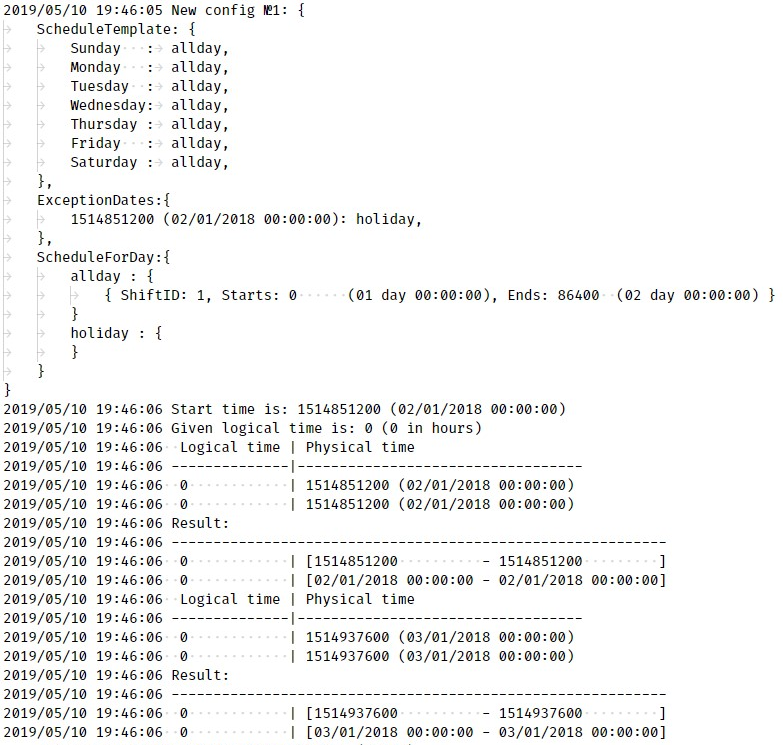
\includegraphics[scale=0.6]{pics/scheduleCheckDateEval.png}
% 	\caption{Пример анализа заданного физического времени}
% 	\label{fig:checkEval}
% \end{figure}

\begin{lstlisting}[caption={Пример анализа заданного физического времени},label={lst:checkEval}]
	2019/05/31 15:12:07 Start time is: 1515326580 (07/01/2018 12:03:00)
	2019/05/31 15:12:07 Given logical time is: 0 (0 in hours)
	2019/05/31 15:12:07  Logical time | Physical time
	2019/05/31 15:12:07 --------------|----------------------------------
	2019/05/31 15:12:07  0            | 1515196800 (06/01/2018 00:00:00)
	2019/05/31 15:12:07  0            | 1515196800 (06/01/2018 00:00:00)
	2019/05/31 15:12:07 Result:
	2019/05/31 15:12:07 -----------------------------------------------------------
	2019/05/31 15:12:07  0     | [1515196800          - 1515196800         ]
	2019/05/31 15:12:07  0     | [06/01/2018 00:00:00 - 06/01/2018 00:00:00]
	2019/05/31 15:12:07  Logical time | Physical time
	2019/05/31 15:12:07 --------------|----------------------------------
	2019/05/31 15:12:07  0            | 1515369600 (08/01/2018 00:00:00)
	2019/05/31 15:12:07  0            | 1515369600 (08/01/2018 00:00:00)
	2019/05/31 15:12:07 Result:
	2019/05/31 15:12:07 -----------------------------------------------------------
	2019/05/31 15:12:07  0     | [1515369600          - 1515369600         ]
	2019/05/31 15:12:07  0     | [08/01/2018 00:00:00 - 08/01/2018 00:00:00]
	--- PASS: TestStartOnWeekendWithZero (0.06s)
	PASS
	ok  	nitta.io/yamp/schedule	0.594s
	Success: Tests passed.
\end{lstlisting}

\indent В результате проведенного тестирования (40 тестов), покрытие кода составило 96.6\%, что отражено в листинге \ref{lst:pass}.

\begin{lstlisting}[caption={Тестовое покрытие кода},label={lst:pass}]
	PASS
	coverage: 96.6% of statements
	ok  	nitta.io/yamp/schedule	0.974s	coverage: 96.6% of statements
	Success: Tests passed.
\end{lstlisting}
